\documentclass[10pt]{beamer}

\usetheme{metropolis}
\usepackage{appendixnumberbeamer}

\usepackage{booktabs}
\usepackage[scale=2]{ccicons}

\usepackage{pgfplots}
\usepgfplotslibrary{dateplot}

\usepackage{xspace}
\newcommand{\themename}{\textbf{\textsc{metropolis}}\xspace}

\title{Internship's progress}
\subtitle{Second presentation}
\date{\today}
\author{Johyn Papin}
\institute{National Institute of Informatics}
% \titlegraphic{\hfill\includegraphics[height=1.5cm]{logo.pdf}}

\begin{document}

\maketitle

\begin{frame}{Table of contents}
  \setbeamertemplate{section in toc}[sections numbered]
  \tableofcontents[hideallsubsections]
\end{frame}

\section{Introduction}

\begin{frame}{Summary Diagram}
    \begin{tikzpicture}[remember picture,overlay]
        \node[at=(current page.center)] {
            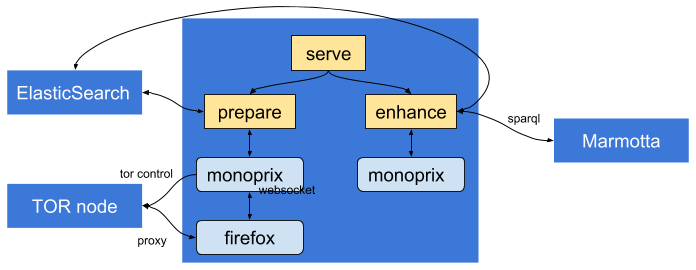
\includegraphics[width=\paperwidth]{summary_diagram.png}
        };
    \end{tikzpicture}
\end{frame}

\section{Progress}

\begin{frame}{Since the last time}
    Here is what has been completed:
	\begin{itemize}
	    \item Tests and docs
		\item Everything is on docker
	    \item ElasticSearch is used to index the monoprix data
	    \begin{itemize}
	        \item indexing with two analyzers: standard and french
	        \item run in docker: performing an index reset is easy
	    \end{itemize}
	    \item Sparql is used to query the triples
	    \begin{itemize}
	        \item backend-independent
	    \end{itemize}
	    \item These triples are enhanced by querying ElasticSearch (match query)
	    \begin{itemize}
	        \item Using an Enhancer interface with the following methods:
	        \begin{itemize}
	            \item \texttt{Next(triple) -> triples}
	            \item \texttt{End() -> triples}
	            \item \texttt{Set(key, value)} and \texttt{Get(key) -> value} for the settings
	        \end{itemize}
	        \item Very easy to add another enhancer (modular)
	        \item Can be filled by a stream of triples
	    \end{itemize}
	\end{itemize}
\end{frame}

\begin{frame}{What I'm doing}
    Here is what I'm doing now:
    \begin{itemize}
        \item Tests and docs
        \item Be able to add the new triples on marmotta via sparql
        \item The web panel
        \begin{itemize}
            \item Must not slow down the rest
            \item Adding a middleware in the log system
            \item Opening a websocket server + a tiny restful API
            \item Using Vue.js:
            \begin{itemize}
                \item incrementally adoptable
                \item tiny
                \item M-V-VM
            \end{itemize}
        \end{itemize}
    \end{itemize}
\end{frame}

\section{Panel design}

\begin{frame}{Login Page}
    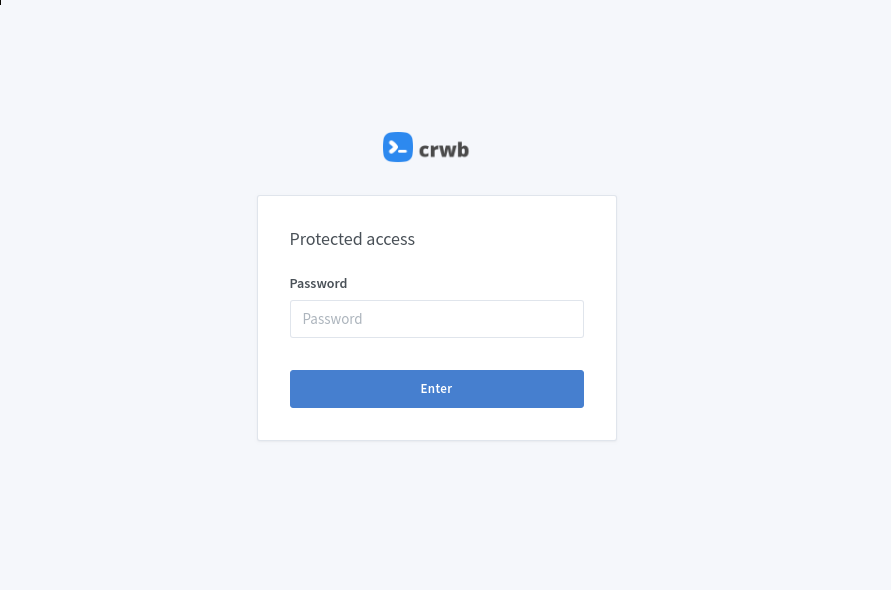
\includegraphics[width=11 cm]{login.png}
\end{frame}


\begin{frame}{Preparation Page}
    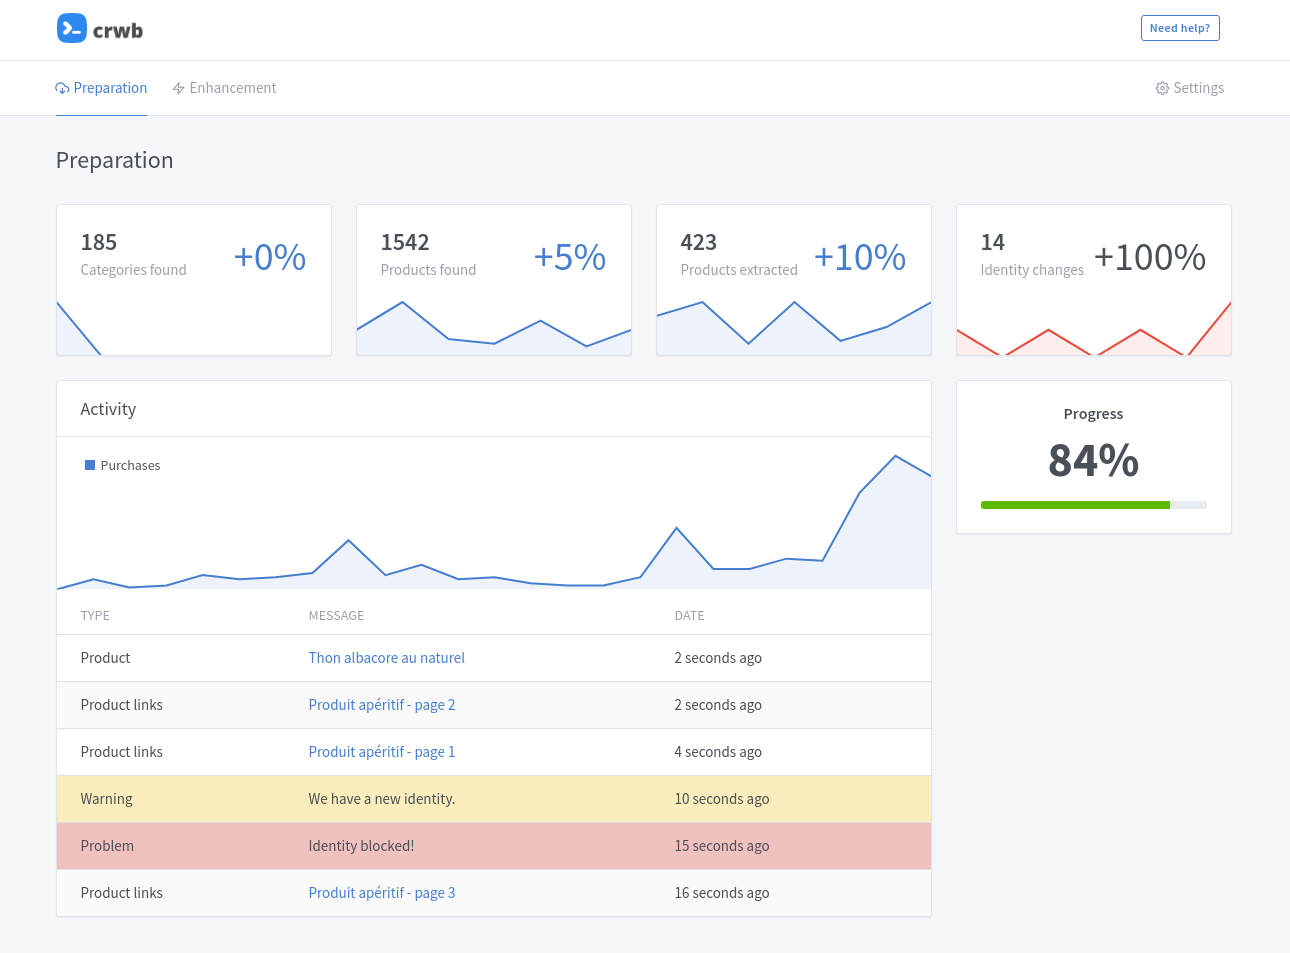
\includegraphics[width=11cm]{preparation.png}
\end{frame}

\section{Conclusion}

\begin{frame}{Summary}

  Get the source of this presentation on

  \begin{center}\url{github.com/johynpapin/yuuri}\end{center}

  The presentation \emph{itself} is licensed under a
  \href{http://creativecommons.org/licenses/by-sa/4.0/}{Creative Commons
  Attribution-ShareAlike 4.0 International License}.

  \begin{center}\ccbysa\end{center}

\end{frame}

\begin{frame}[standout]
  Questions?
\end{frame}

\appendix

\end{document}

